\chapter{Análise dos Resultados}
\label{cap:resultados}
Os testes para \textit{Serie-PH} nos mostram intervalos de latência bastante consistentes com diferença entre os extremos suficientemente restrita, como nos mostram a tabela \ref{serie-phTabela}. Podemos dizer que quanto mais restrito o intervalo de valores mais previsível é o sistema. Na maior parte das tarefas executadas tanto no Preempt\_RT, que registrou latências menores, quanto no RTAI, intervalos mais estreitos (figura \ref{serie-phPRTvsRTAI}), com exceção da \textit{thread} 4 do teste executado no RTAI na qual fica evidente a existência de uma anomalia, e que ainda não teve sua causa identificada.

\begin{figure}[!h]
    \centering
    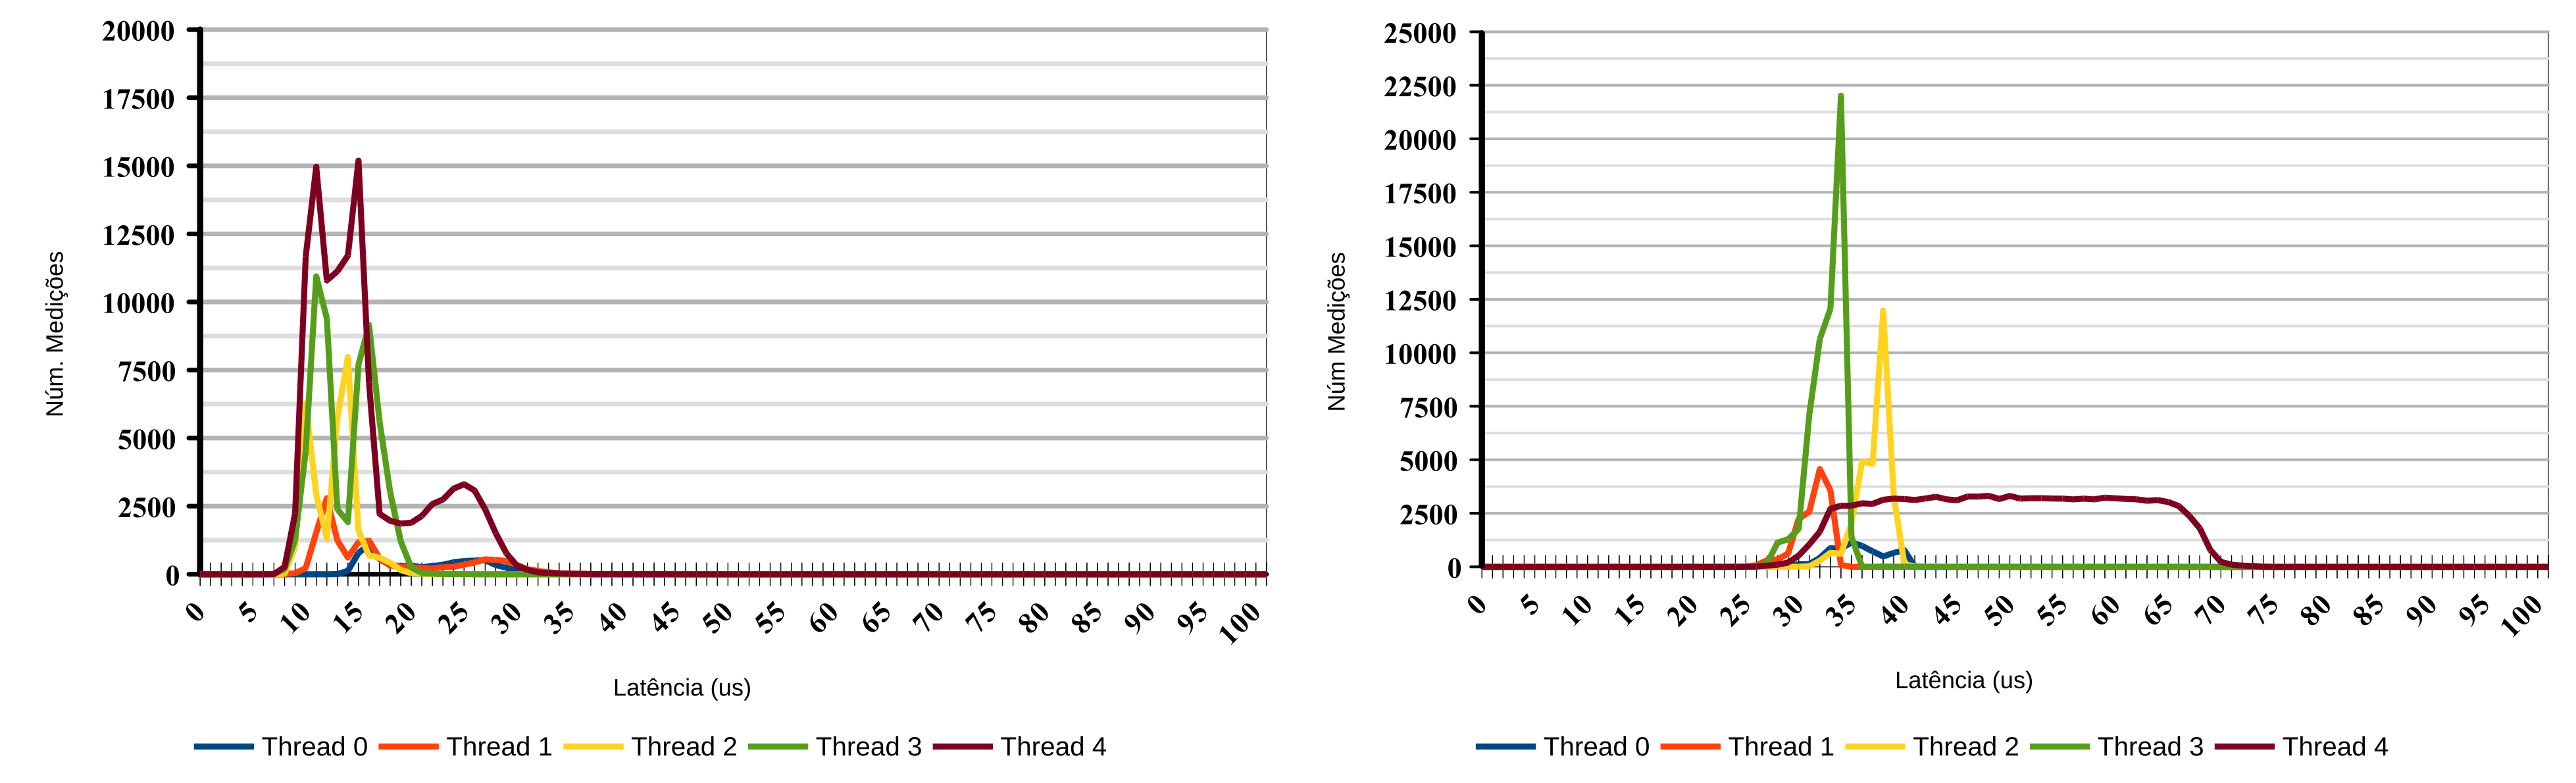
\includegraphics[scale=0.95]{serie-phPRTvsRTAI}
    \caption{Medidas de latência dos testes \textit{Serie-PH} - Preempt\_RT x RTAI}
    \label{serie-phPRTvsRTAI}
\end{figure}

Embora estejam distribuídos de forma  adequada, os valores máximos de latência, em alguns casos, superam 100\% do tempo de computação máximo das tarefas (tabela \ref{TcTabela}) o que pode ser um grande problema para tarefas com \textit{deadlines} na casa dos microssegundos, porém para as tarefas executadas, a soma dos valores de Latência e Tempo de Computação foram bem inferior aos deadlines definidos.

Quando adicionamos duas tarefas aperiódicas aos testes (\textit{Serie-AH}) e observamos os histogramas na figura \ref{serie-ahPRTvsRTAI}, podemos visualizar alguns comportamentos interessantes. A execução das tarefas pelo \textit{patch} Preempt\_RT a primeira vista se mostraram inalteradas, mas uma análise detalhada dos valores de latência mostram alguns pontos fora da curva e registros de latência máxima bem superiores a maioria das medições feitas nos testes da da \textit{Serie-PH}, embora os valores não tenham comprometido a execução da aplicação, a soma dos valores de latência e tempo de computação ainda foram bem inferiores ao \textit{deadline}, esse tipo de comportamento imprevisível reforça a necessidade de testes de medição de latência com a aplicação pretendida. 

\begin{figure}[!h]
    \centering
    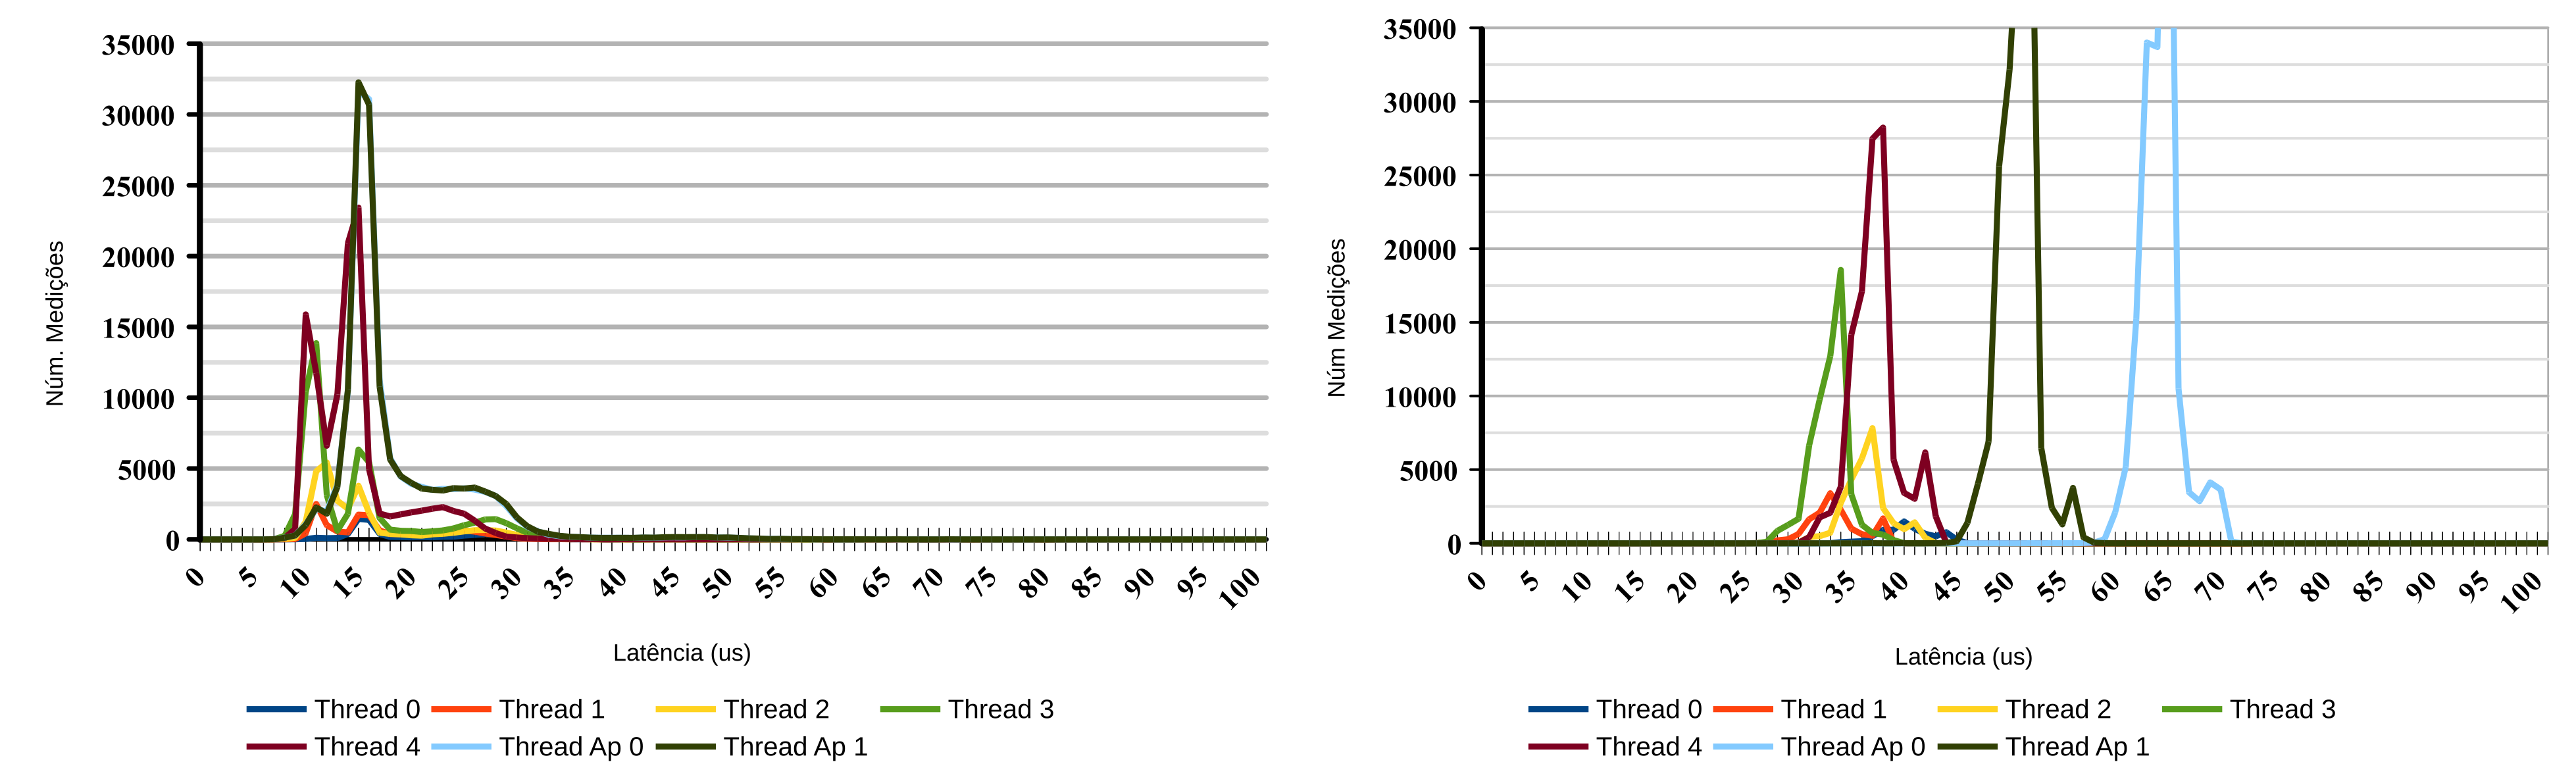
\includegraphics[scale=0.95]{serie-ahPRTvsRTAI}
    \caption{Medidas de latência dos testes \textit{Serie-AH} - Preempt\_RT x RTAI}
    \label{serie-ahPRTvsRTAI}
\end{figure}

A coluna para os testes \textit{Serie-AH} da tabela \ref{TcTabela} nos mostra que os valores dos tempos de computação para o Preempt\_RT foram praticamente 100\% maiores que os valores medidos para os testes com a \textit{Serie-PH}, embora mais uma vez os deadlines foram respeitados. Já o RTAI não teve qualquer alteração nos valores de latência e nos valores do tempo de computação para as atividades periódicas, porém na figura \ref{serie-ahPRTvsRTAI} podemos ver um comportamento que tende a adiar a execução das tarefas aperiódicas ao longo do tempo, embora os valores tenha estado dentro de um intervalo bem definido e as curvas serem muito parecidas, podemos nos questionar se a adição de novas tarefas aperiódicas provocaria o aumento das latências destas tarefas.

A análise dos valores medidos para latências a que as tarefas de tempo real estão sujeitas e dos seus respectivos tempos de computação nos mostram que, tanto o Preempt\_RT quanto o RTAI, podem executar com segurança, tarefas de tempo real com restrições temporais na casa dos milissegundos. Para sistemas que possuam tarefas com restrições temporais na menores que 1ms e recomendada, além da execução de testes de validação dentro da própria aplicação, o projeto cuidadoso do escalonamento das tarefas, com especial atenção a atribuição da prioridades, caso seja utilizado um escalonador FIFO ou RM.

Ao compararmos os valores obtidos com os resultados apresentados na tabela \ref{CompTabela}, fornecidos por \cite{Anderson2007}, que aplicou testes semelhantes ao RTAI, e \cite{Litayem2011}, que utilizou o \textit{benchmark Cyclictest} para medir a latência no Preempt\_RT, podemos dizer que, embora tenham sido um pouco mais altos, mostram que o comportamento dos sistemas ante a heterogeneidade dos métodos de análise, testes aplicados e hardwares utilizados, esteve dentro do esperado e com uma variação de valores relativamente pequena o que seria esperado já que as principais funcionalidades de um SOTR é abstrair o comportamento do hardware e apresentar ao desenvolvedor uma camada de abstração consistente, independente da situação em que se encontra o sistema, sobre a qual possam desenvolver suas aplicações de forma previsível.

\begin{table}[!h]
\centering
\begin{tabular}{c|c|c|c|c|}
\cline{2-5} 
 & \multicolumn{2}{c|}{Preempt\_RT} & \multicolumn{2}{c|}{RTAI} \\ 
\hline 
\multicolumn{1}{ |c| }{\textit{Thread}} & Latência Máx. & Latência Mín. & Latência Máx. & Latência Mín. \\ 
\hline 
\multicolumn{1}{ |c| }{0} & 39 & 13 & 41 & 28 \\ 
\hline 
\multicolumn{1}{ |c| }{1} & 43 & 8 & 38 & 22 \\ 
\hline 
\multicolumn{1}{ |c| }{2} & 30 & 8 & 44 & 27 \\ 
\hline 
\multicolumn{1}{ |c| }{3} & 25 & 7 & 40 & 24 \\ 
\hline 
\multicolumn{1}{ |c| }{4} & 44 & 7 & 74 & 20 \\ 
\hline 
\end{tabular} 
\caption{Valores (em \si{\micro\s}) máximos e mínimos de latência obtidos nos testes \textit{Serie-PH}- Preempt\_RT x RTAI}
\label{serie-phTabela}
\end{table}

\begin{table}[!h]
\centering
\begin{tabular}{c|c|c|c|c|}
\cline{2-5} 
 & \multicolumn{2}{c|}{Preempt\_RT} & \multicolumn{2}{c|}{RTAI} \\ 
\hline 
\multicolumn{1}{ |c| }{\textit{Thread}} & Latência Máx. & Latência Mín. & Latência Máx. & Latência Mín. \\ 
\hline 
\multicolumn{1}{ |c| }{0} & 70 & 9 & 46 & 32 \\ 
\hline 
\multicolumn{1}{ |c| }{1} & 72 & 8 & 39 & 25 \\ 
\hline 
\multicolumn{1}{ |c| }{2} & 71 & 7 & 43 & 28 \\ 
\hline 
\multicolumn{1}{ |c| }{3} & 74 & 7 & 39 & 21 \\ 
\hline 
\multicolumn{1}{ |c| }{4} & 67 & 7 & 45 & 23 \\ 
\hline 
\multicolumn{1}{ |c| }{Ap. 0} & 80 & 6 & 72 & 52 \\ 
\hline 
\multicolumn{1}{ |c| }{Ap. 1} & 71 & 7 & 59 & 37 \\ 
\hline 
\end{tabular} 
\caption{Valores (em \si{\micro\s}) máximos e mínimos de latência obtidos nos testes \textit{Serie-AH}- Preempt\_RT x RTAI}
\label{serie-ahTabela}
\end{table}

\begin{table}[!th]
\centering
\begin{tabular}{c|c|c|c|c|}
\cline{2-5} 
 & \multicolumn{2}{c|}{Preempt\_RT} & \multicolumn{2}{c|}{RTAI} \\ 
\hline 
\multicolumn{1}{ |c| }{\textit{Thread}} & Tc (\textit{Serie-PH}) & Tc (\textit{Serie-AH}) & Tc (\textit{Serie-PH}) & Tc (\textit{Serie-AH}) \\ 
\hline 
\multicolumn{1}{ |c| }{0} & 18 & 70 & 19 & 21 \\ 
\hline 
\multicolumn{1}{ |c| }{1} & 38 & 81 & 45 & 45 \\ 
\hline 
\multicolumn{1}{ |c| }{2} & 39 & 83 & 37 & 36 \\ 
\hline 
\multicolumn{1}{ |c| }{3} & 27 & 70 & 28 & 20 \\ 
\hline 
\multicolumn{1}{ |c| }{4} & 39 & 79 & 43 & 40 \\ 
\hline 
\multicolumn{1}{ |c| }{Ap. 0} & - & 62 & - & 42 \\ 
\hline 
\multicolumn{1}{ |c| }{Ap. 1} & - & 56 & - & 44 \\ 
\hline 
\end{tabular} 
\caption{Valores (em \si{\micro\s}) do tempo de computação máximo obtidos nos testes \textit{Serie-PH} e \textit{Serie-AH} - Preempt\_RT x RTAI}
\label{TcTabela}
\end{table}

\begin{table}[!h]
\centering
\begin{tabular}{|c|c|c|}
\hline 
\multicolumn{2}{|c|}{RTAI \cite{Anderson2007}} & Preempt\_RT \cite{Litayem2011}\\ 
\hline 
Latência & Tc & Latência \\ 
\hline 
3 & 34 a 47 & 7 a 62 \\ 
\hline 
\end{tabular} 
\caption{Valores (em \si{\micro\s}) de latência e tempo de computação obtidos por \cite{Anderson2007} e \cite{Litayem2011}}
\label{CompTabela}
\end{table}

